% Options for packages loaded elsewhere
% Options for packages loaded elsewhere
\PassOptionsToPackage{unicode}{hyperref}
\PassOptionsToPackage{hyphens}{url}
%
\documentclass[
  ignorenonframetext,
  aspectratio=169,
  russian,
]{beamer}
\newif\ifbibliography
\usepackage{pgfpages}
\setbeamertemplate{caption}[numbered]
\setbeamertemplate{caption label separator}{: }
\setbeamercolor{caption name}{fg=normal text.fg}
\beamertemplatenavigationsymbolshorizontal
% remove section numbering
\setbeamertemplate{part page}{
  \centering
  \begin{beamercolorbox}[sep=16pt,center]{part title}
    \usebeamerfont{part title}\insertpart\par
  \end{beamercolorbox}
}
\setbeamertemplate{section page}{
  \centering
  \begin{beamercolorbox}[sep=12pt,center]{section title}
    \usebeamerfont{section title}\insertsection\par
  \end{beamercolorbox}
}
\setbeamertemplate{subsection page}{
  \centering
  \begin{beamercolorbox}[sep=8pt,center]{subsection title}
    \usebeamerfont{subsection title}\insertsubsection\par
  \end{beamercolorbox}
}
% Prevent slide breaks in the middle of a paragraph
\widowpenalties 1 10000
\raggedbottom
\AtBeginPart{
  \frame{\partpage}
}
\AtBeginSection{
  \ifbibliography
  \else
    \frame{\sectionpage}
  \fi
}
\AtBeginSubsection{
  \frame{\subsectionpage}
}
\usepackage{iftex}
\ifPDFTeX
  \usepackage[T1]{fontenc}
  \usepackage[utf8]{inputenc}
  \usepackage{textcomp} % provide euro and other symbols
\else % if luatex or xetex
  \usepackage{unicode-math} % this also loads fontspec
  \defaultfontfeatures{Scale=MatchLowercase}
  \defaultfontfeatures[\rmfamily]{Ligatures=TeX,Scale=1}
\fi
\usepackage{lmodern}

\usetheme[]{metropolis}
\usefonttheme{serif} % use mainfont rather than sansfont for slide text
\ifPDFTeX\else
  % xetex/luatex font selection
  \setmainfont[]{DejaVu Sans}
  \setsansfont[]{DejaVu Sans}
  \setmonofont[]{DejaVu Sans Mono}
\fi
% Use upquote if available, for straight quotes in verbatim environments
\IfFileExists{upquote.sty}{\usepackage{upquote}}{}
\IfFileExists{microtype.sty}{% use microtype if available
  \usepackage[]{microtype}
  \UseMicrotypeSet[protrusion]{basicmath} % disable protrusion for tt fonts
}{}


\usepackage{longtable,booktabs,array}
\newcounter{none} % for unnumbered tables
\usepackage{calc} % for calculating minipage widths
\usepackage{caption}
% Make caption package work with longtable
\makeatletter
\def\fnum@table{\tablename~\thetable}
\makeatother
\usepackage{graphicx}
\makeatletter
\newsavebox\pandoc@box
\newcommand*\pandocbounded[1]{% scales image to fit in text height/width
  \sbox\pandoc@box{#1}%
  \Gscale@div\@tempa{\textheight}{\dimexpr\ht\pandoc@box+\dp\pandoc@box\relax}%
  \Gscale@div\@tempb{\linewidth}{\wd\pandoc@box}%
  \ifdim\@tempb\p@<\@tempa\p@\let\@tempa\@tempb\fi% select the smaller of both
  \ifdim\@tempa\p@<\p@\scalebox{\@tempa}{\usebox\pandoc@box}%
  \else\usebox{\pandoc@box}%
  \fi%
}
% Set default figure placement to htbp
\def\fps@figure{htbp}
\makeatother



\ifLuaTeX
\usepackage[bidi=basic,shorthands=off,provide=*]{babel}
\else
\usepackage[bidi=default,shorthands=off,provide=*]{babel}
\fi
\ifPDFTeX
\else
\babelfont{rm}[]{DejaVu Sans}
\fi
\ifLuaTeX
  \usepackage{selnolig} % disable illegal ligatures
\fi


\setlength{\emergencystretch}{3em} % prevent overfull lines

\providecommand{\tightlist}{%
  \setlength{\itemsep}{0pt}\setlength{\parskip}{0pt}}



 

\usepackage[]{csquotes}

%%% Load theme
\IfFileExists{beamerthemegotham.sty}{
  %%%% Full TeXlive
  \usetheme{gotham}
  \gothamset{
    numbering=totalframenumber,
    parttocframe default=off,
    sectiontocframe default=off,
    subsectiontocframe default=off,
    tocframe template=gotham bullet,
    % progressbar position=frametitle,
    progressbar position=foot,
  }
  \renewcommand{\gothamInstituteLogoSquare}[1][4ex]{%
    
\includegraphics[height=##1]{_resources/image/logo_rudn-inverted.png}
  }
  % \renewcommand{\gothamtitlepagelogo}[1][4ex]{%
  %   
\includegraphics[height=##1]{_resources/image/logo_rudn.png}
  % }
}{%
  %%%% TinyTeX
  \usepackage{libertine}
  %%%% https://deic.uab.cat/~iblanes/beamer_gallery/
  \usetheme{Madrid}
}
\metroset{progressbar=frametitle,numbering=fraction}
\makeatletter
\@ifpackageloaded{caption}{}{\usepackage{caption}}
\AtBeginDocument{%
\ifdefined\contentsname
  \renewcommand*\contentsname{Содержание}
\else
  \newcommand\contentsname{Содержание}
\fi
\ifdefined\listfigurename
  \renewcommand*\listfigurename{Список иллюстраций}
\else
  \newcommand\listfigurename{Список иллюстраций}
\fi
\ifdefined\listtablename
  \renewcommand*\listtablename{Список таблиц}
\else
  \newcommand\listtablename{Список таблиц}
\fi
\ifdefined\figurename
  \renewcommand*\figurename{Рисунок}
\else
  \newcommand\figurename{Рисунок}
\fi
\ifdefined\tablename
  \renewcommand*\tablename{Таблица}
\else
  \newcommand\tablename{Таблица}
\fi
}
\@ifpackageloaded{float}{}{\usepackage{float}}
\floatstyle{ruled}
\@ifundefined{c@chapter}{\newfloat{codelisting}{h}{lop}}{\newfloat{codelisting}{h}{lop}[chapter]}
\floatname{codelisting}{Список}
\newcommand*\listoflistings{\listof{codelisting}{Листинги}}
\makeatother
\makeatletter
\makeatother
\makeatletter
\@ifpackageloaded{caption}{}{\usepackage{caption}}
\@ifpackageloaded{subcaption}{}{\usepackage{subcaption}}
\makeatother

\usepackage{bookmark}
\IfFileExists{xurl.sty}{\usepackage{xurl}}{} % add URL line breaks if available
\urlstyle{same}
% fallback for those not using the hyperref driver hyperxmp:
\makeatletter
\@ifundefined{xmpquote}{\newcommand{\xmpquote}[1]{#1}}{}
\makeatother
\hypersetup{
  pdftitle={Лабораторная работа №4},
  pdfauthor={Нечаева Кира Андреевна},
  pdflang={ru-RU},
  hidelinks,
  pdfcreator={LaTeX via pandoc}}


\title{\texorpdfstring{Лабораторная работа №4}{Лабораторная работа №4}}
\subtitle{\texorpdfstring{Модель гармонического
осциллятора}{Модель гармонического осциллятора}}
\author{Нечаева Кира Андреевна}
\date{}
\institute{НКНбд-01-23}

\begin{document}
\frame{\titlepage}


\begin{frame}{Постановка задачи}
\protect\phantomsection\label{ux43fux43eux441ux442ux430ux43dux43eux432ux43aux430-ux437ux430ux434ux430ux447ux438}
\textbf{Вариант 2}

Начальные условия:

\[
x(0)=1,\qquad x'(0)=1.
\]

Интервал:

\[
t\in[0;40],\qquad \Delta t=0.05.
\]

Исследуются три режима:

\begin{itemize}
\tightlist
\item
  без затухания;
\item
  с затуханием;
\item
  с затуханием и внешней силой.
\end{itemize}
\end{frame}

\begin{frame}{Численное решение}
\protect\phantomsection\label{ux447ux438ux441ux43bux435ux43dux43dux43eux435-ux440ux435ux448ux435ux43dux438ux435}
Уравнение второго порядка представляется системой:

\[
x'=y,
\]

\[
y'=f(t,x,y).
\]

После этого система численно решается в Julia.

Для каждого случая строятся:

\begin{itemize}
\tightlist
\item
  решение \(x(t)\);
\item
  фазовый портрет \((x,x')\).
\end{itemize}
\end{frame}

\begin{frame}{Случай 1. Без затухания}
\protect\phantomsection\label{ux441ux43bux443ux447ux430ux439-1.-ux431ux435ux437-ux437ux430ux442ux443ux445ux430ux43dux438ux44f}
\[
x''+3x=0
\]

или

\[
x'=y,\qquad y'=-3x.
\]

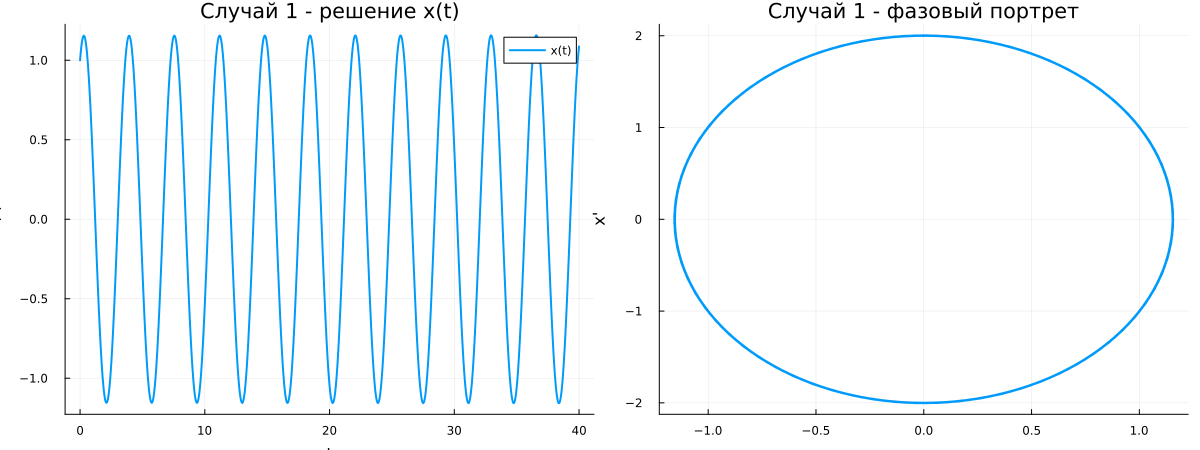
\includegraphics[width=0.88\linewidth,height=\textheight,keepaspectratio]{image/case1_combined.png}

Амплитуда колебаний сохраняется.

Фазовая траектория замкнута.
\end{frame}

\begin{frame}{Случай 2. С затуханием}
\protect\phantomsection\label{ux441ux43bux443ux447ux430ux439-2.-ux441-ux437ux430ux442ux443ux445ux430ux43dux438ux435ux43c}
\[
x''+x'+4x=0
\]

или

\[
x'=y,\qquad y'=-y-4x.
\]

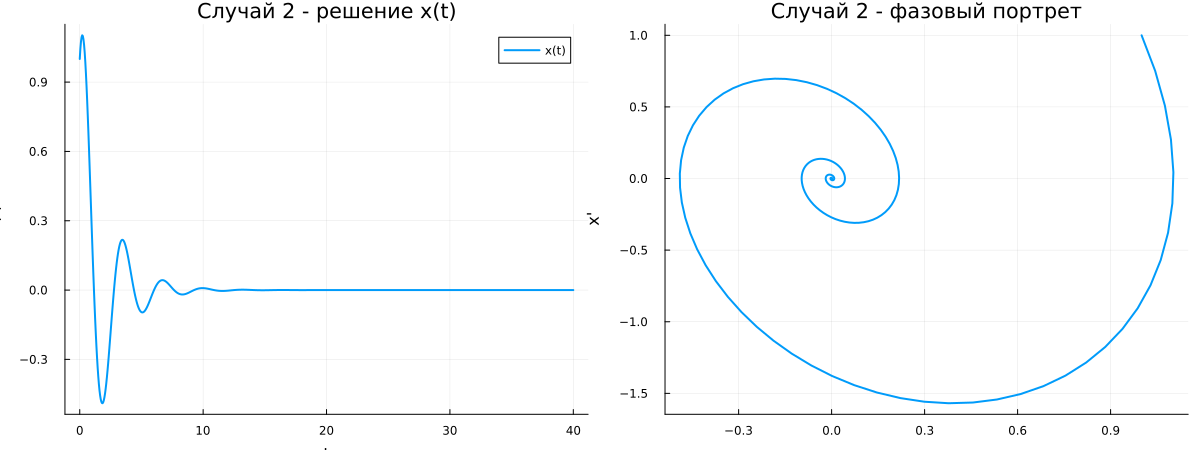
\includegraphics[width=0.88\linewidth,height=\textheight,keepaspectratio]{image/case2_combined.png}

Амплитуда со временем уменьшается.
\end{frame}

\begin{frame}{Что меняется при затухании}
\protect\phantomsection\label{ux447ux442ux43e-ux43cux435ux43dux44fux435ux442ux441ux44f-ux43fux440ux438-ux437ux430ux442ux443ux445ux430ux43dux438ux438}
В системе появляется член, зависящий от скорости:

\[
-y.
\]

Он описывает потери энергии.

Поэтому:

\begin{itemize}
\tightlist
\item
  колебания постепенно ослабевают;
\item
  решение стремится к нулю;
\item
  фазовая траектория приближается к началу координат.
\end{itemize}
\end{frame}

\begin{frame}{Случай 3. Внешняя сила}
\protect\phantomsection\label{ux441ux43bux443ux447ux430ux439-3.-ux432ux43dux435ux448ux43dux44fux44f-ux441ux438ux43bux430}
\[
x''+2x'+x=\sin(2t)
\]

или

\[
x'=y,
\]

\[
y'=\sin(2t)-2y-x.
\]

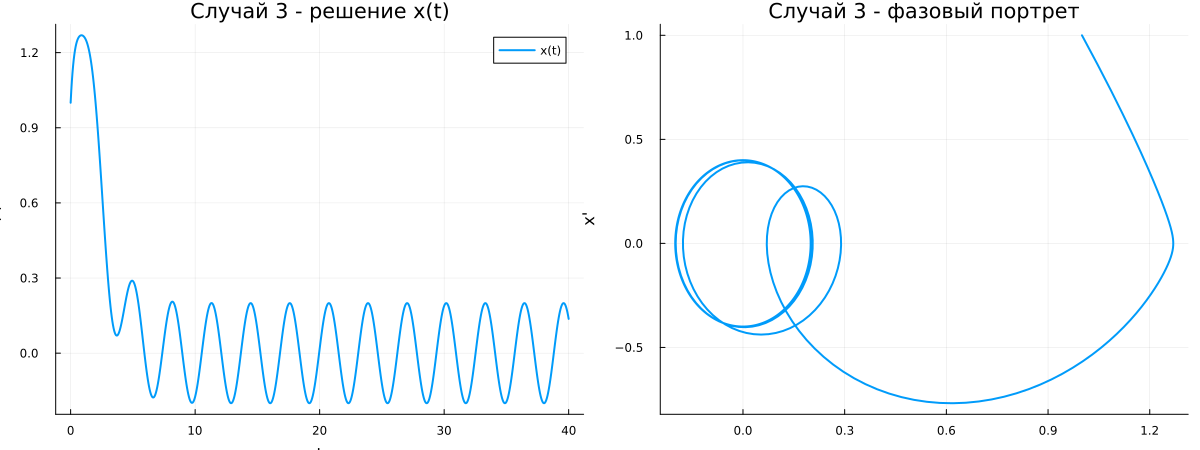
\includegraphics[width=0.88\linewidth,height=\textheight,keepaspectratio]{image/case3_combined.png}
\end{frame}

\begin{frame}{Роль внешней силы}
\protect\phantomsection\label{ux440ux43eux43bux44c-ux432ux43dux435ux448ux43dux435ux439-ux441ux438ux43bux44b}
Внешнее воздействие

\[
\sin(2t)
\]

периодически передаёт системе энергию.

Поэтому, несмотря на затухание, колебания не исчезают полностью.

После переходного процесса движение поддерживается внешней силой.
\end{frame}

\begin{frame}{Сравнение}
\protect\phantomsection\label{ux441ux440ux430ux432ux43dux435ux43dux438ux435}
\textbf{Без затухания}

Амплитуда сохраняется.

\textbf{С затуханием}

Амплитуда уменьшается.

\textbf{С внешней силой}

Колебания продолжаются за счёт внешнего воздействия.

Фазовые портреты наглядно показывают различие поведения системы.
\end{frame}

\begin{frame}{Итог}
\protect\phantomsection\label{ux438ux442ux43eux433}
Для варианта 2 исследованы три режима гармонического осциллятора.

Для каждого случая:

\begin{itemize}
\tightlist
\item
  уравнение второго порядка преобразовано в систему первого порядка;
\item
  выполнено численное решение;
\item
  построена зависимость \(x(t)\);
\item
  построен фазовый портрет.
\end{itemize}

Характер движения определяется наличием затухания и внешней силы.
\end{frame}




\end{document}
